\section{Tasks \#1. White correction}
\subsection{Colorchecker [from Specim scanner]}

White correction of specim scanner is shown in Figure \ref{fig:wc-specim-scanner}. 
The white correction is done by using a white reference and a dark reference. 

Script for white correction is shown in Code \ref{code:wc-specim-scanner}.

\begin{figure}[H]
    \centering
    \caption{White correction of specim scanner}
    \label{fig:wc-specim-scanner}
    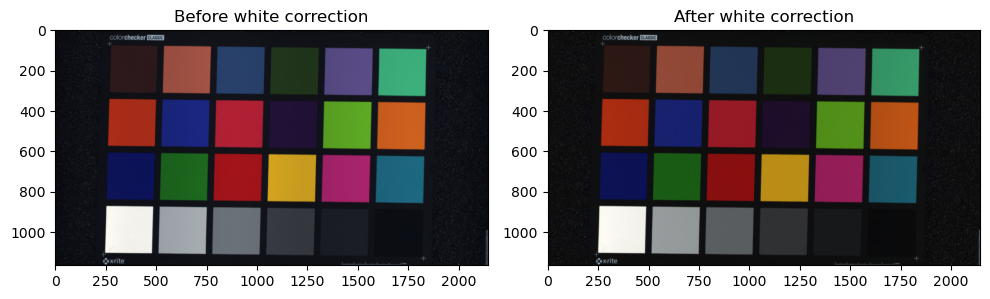
\includegraphics[width=0.75\textwidth]{./fig-task1/specium-scanner.png}
\end{figure}

Spectra of white corrected image is shown in Figure \ref{fig:wc-specim-scanner-spectra}.

\begin{figure}[H]
    \centering
    \caption{Spectra of white corrected image}
    \label{fig:wc-specim-scanner-spectra}
    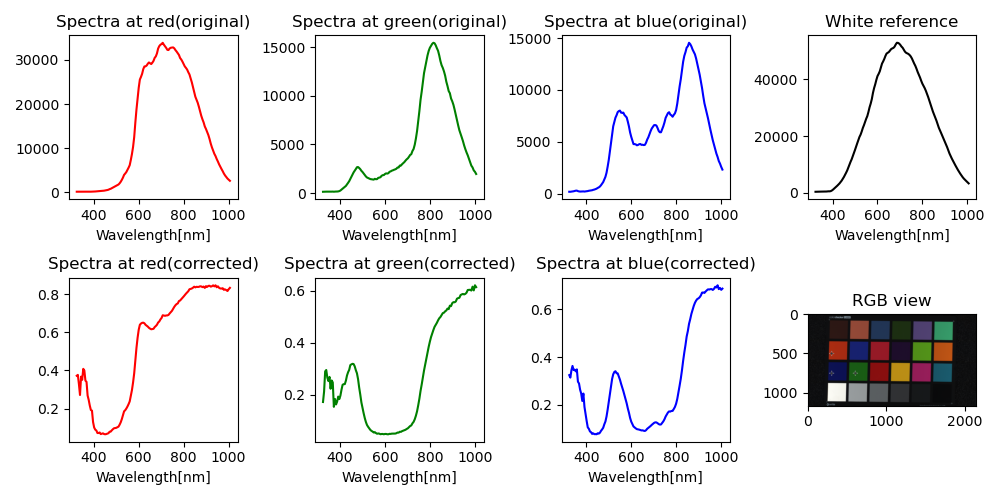
\includegraphics[width=0.75\textwidth]{./fig-task1/wc-specim-scanner-spectra.png}
\end{figure}

\subsection{Color Checker 2 lamps + White Sample 2 lamps}

\subsubsection{SpecimIQ}

White correction of SpecimIQ is shown in Figure \ref{fig:wc-specimiq-large}.

\begin{figure}[H]
    \centering
    \caption{White correction of SpecimIQ with large reference}
    \label{fig:wc-specimiq-large}
    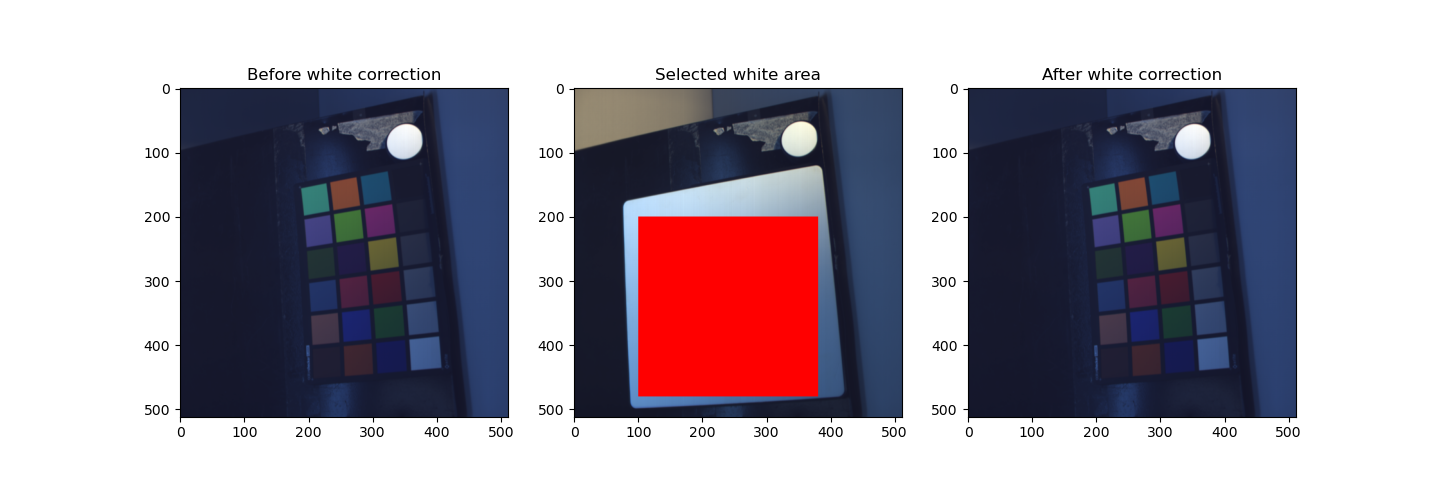
\includegraphics[width=0.75\textwidth]{./fig-task1/wc-specimiq-large.png}
\end{figure}

Spectra of white corrected image is shown in Figure \ref{fig:wc-specimiq-large-spectra}.

\begin{figure}[H]
    \centering
    \caption{Spectra of white corrected image}
    \label{fig:wc-specimiq-large-spectra}
    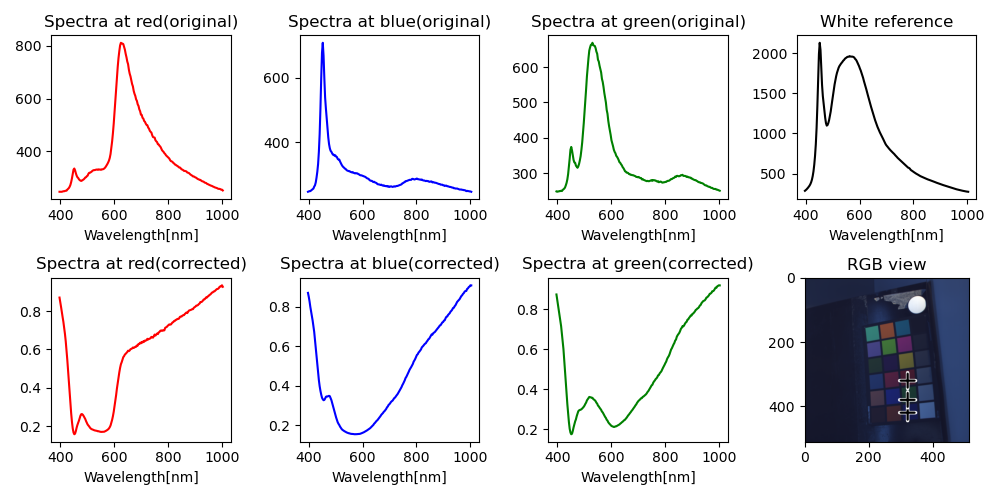
\includegraphics[width=0.75\textwidth]{./fig-task1/wc-specimiq-large-spectra.png}
\end{figure}

Figures were generated with the script shown in Code \ref{code:wc-specimiq-large}.

\subsubsection{Nuance camera}
White correction of nuance camera is shown in Figure \ref{fig:wc-nuance-camera-large}.

\begin{figure}[H]
    \centering
    \caption{White correction of nuance camera with large reference}
    \label{fig:wc-nuance-camera-large}
    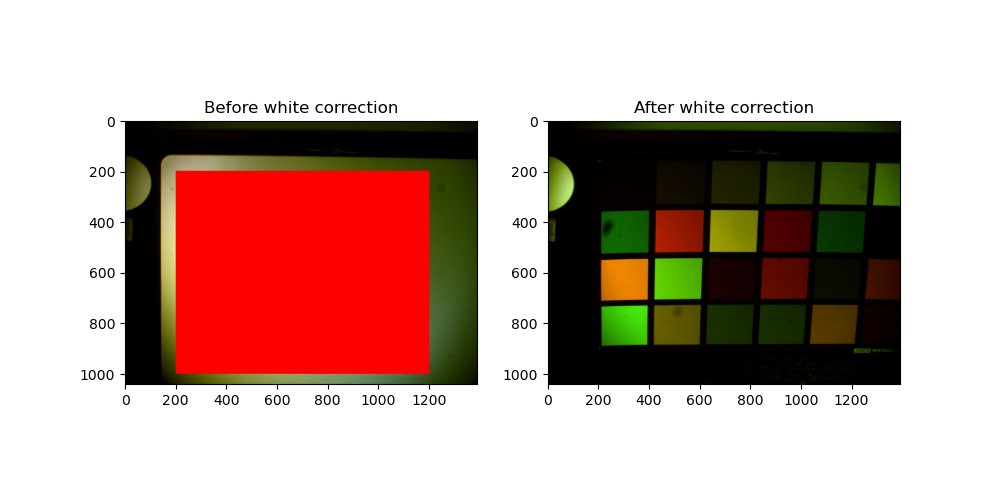
\includegraphics[width=0.75\textwidth]{./fig-task1/wc-nuance-large.png}
\end{figure}

Spectra of white corrected image is shown in Figure \ref{fig:wc-nuance-camera-large-spectra}.

\begin{figure}[H]
    \centering
    \caption{Spectra of white corrected image}
    \label{fig:wc-nuance-camera-large-spectra}
    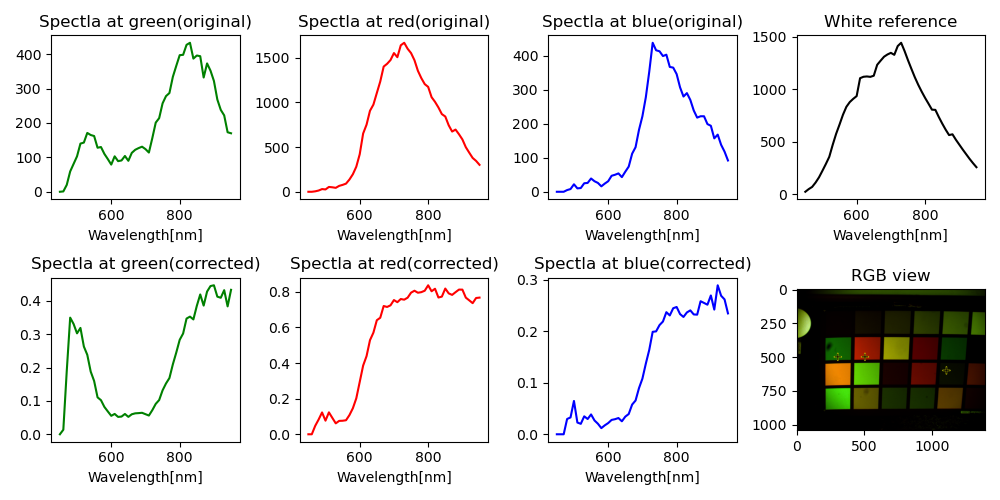
\includegraphics[width=0.75\textwidth]{./fig-task1/wc-nuance-spectra-large.png}
\end{figure}

Nuance image was loaded with the script shown in Code \ref{code:load-nuance}.
Figures were generated with the script shown in Code \ref{code:wc-nuance-large}.


\subsection{Color Checker 2 lamps using left and right white samples inside the image}

\subsubsection{SpecimIQ}
White correction of SpecimIQ is shown in Figure \ref{fig:wc-specimiq-small}.

\begin{figure}[H]
    \centering
    \caption{White correction of SpecimIQ}
    \label{fig:wc-specimiq-small}
    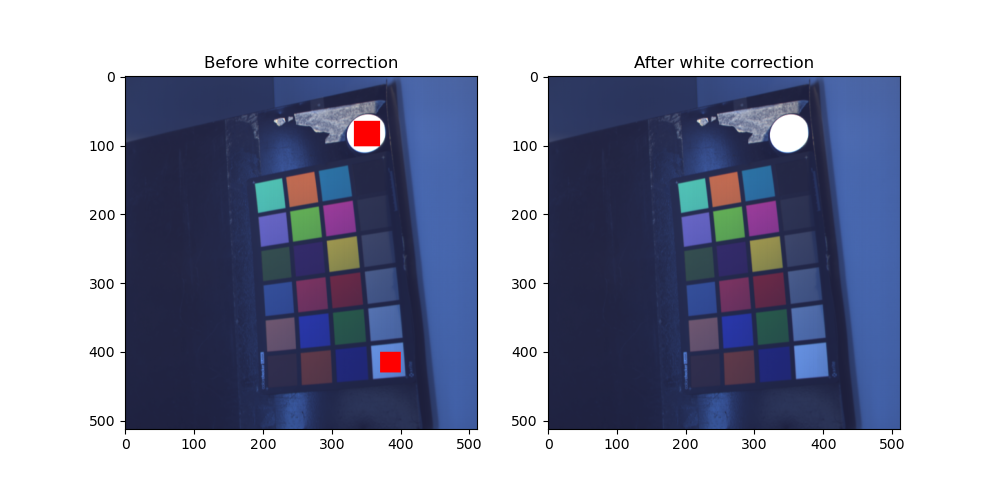
\includegraphics[width=0.75\textwidth]{./fig-task1/wc-specimiq-small.png}
\end{figure}

Spectra of white corrected image is shown in Figure \ref{fig:wc-specimiq-small-spectra}.

\begin{figure}[H]
    \centering
    \caption{Spectra of white corrected image}
    \label{fig:wc-specimiq-small-spectra}
    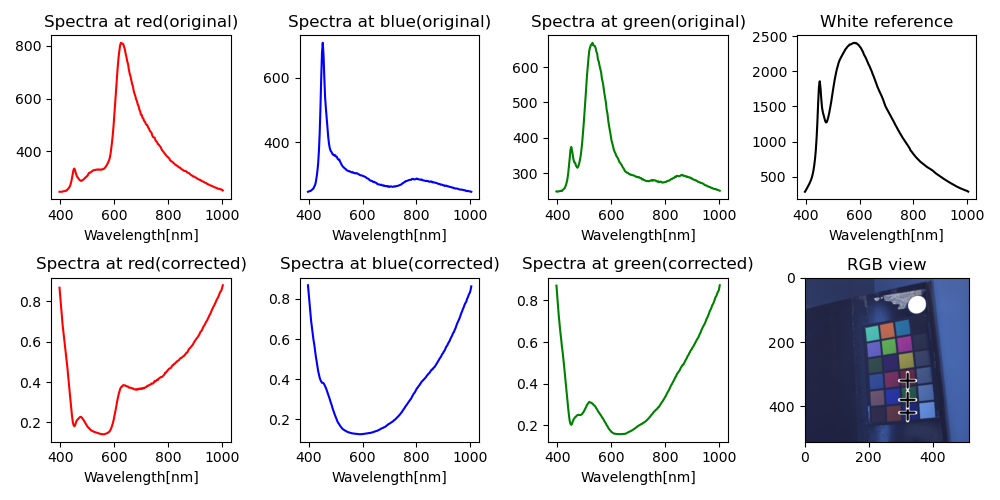
\includegraphics[width=0.75\textwidth]{./fig-task1/wc-specimiq-small-spectra.png}
\end{figure}

Figures were generated with the script shown in Code \ref{code:wc-specimiq-small}.


\subsubsection{Nuance camera}

White correction of nuance camera is shown in Figure \ref{fig:wc-nuance-camera-small}.

\begin{figure}[H]
    \centering
    \caption{White correction of nuance camera}
    \label{fig:wc-nuance-camera-small}
    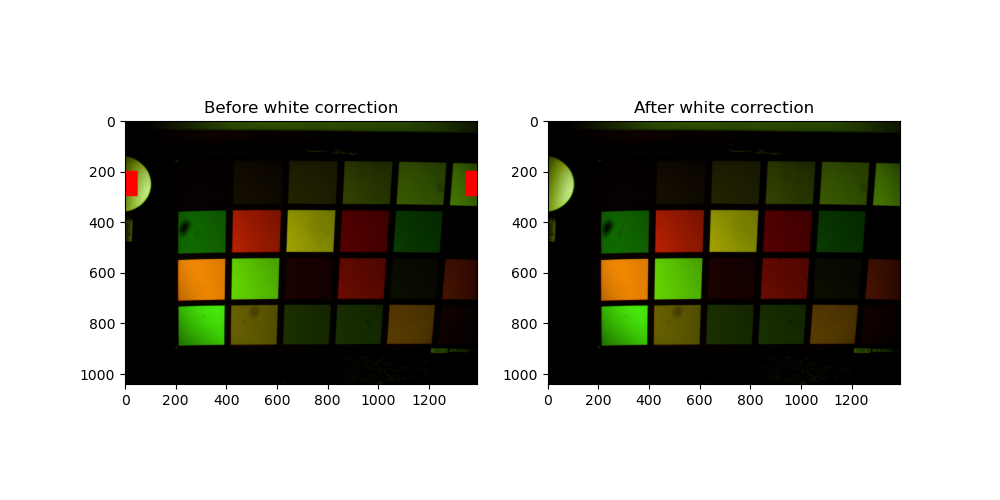
\includegraphics[width=0.75\textwidth]{./fig-task1/wc-nuance-small.png}
\end{figure}

Spectra of white corrected image is shown in Figure \ref{fig:wc-nuance-camera-small-spectra}.

\begin{figure}[H]
    \centering
    \caption{Spectra of white corrected image}
    \label{fig:wc-nuance-camera-small-spectra}
    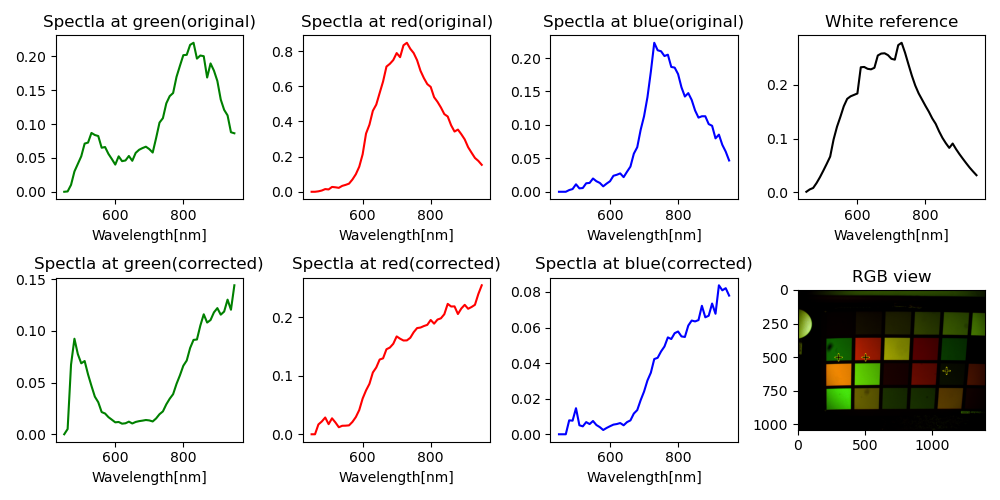
\includegraphics[width=0.75\textwidth]{./fig-task1/wc-nuance-spectra-small.png}
\end{figure}

Nuance image was loaded with the script shown in Code \ref{code:load-nuance}.
Figures were generated with the script shown in Code \ref{code:wc-nuance-small}.


\subsection{Tunable light source}
White correction of tunable light camera is shown in Figure \ref{fig:wc-tunable}.

\begin{figure}[H]
    \centering
    \caption{White correction of tunable light source}
    \label{fig:wc-tunable}
    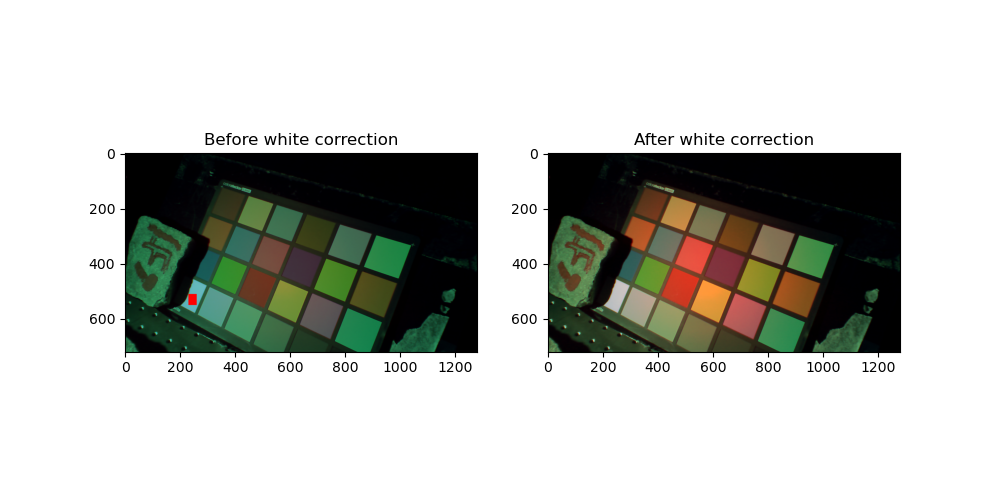
\includegraphics[width=0.75\textwidth]{./fig-task1/wc-tunable.png}
\end{figure}

Spectra of white corrected image is shown in Figure \ref{fig:wc-tunable-spectra}

\begin{figure}[H]
    \centering
    \caption{Spectra of white corrected image}
    \label{fig:wc-tunable-spectra}
    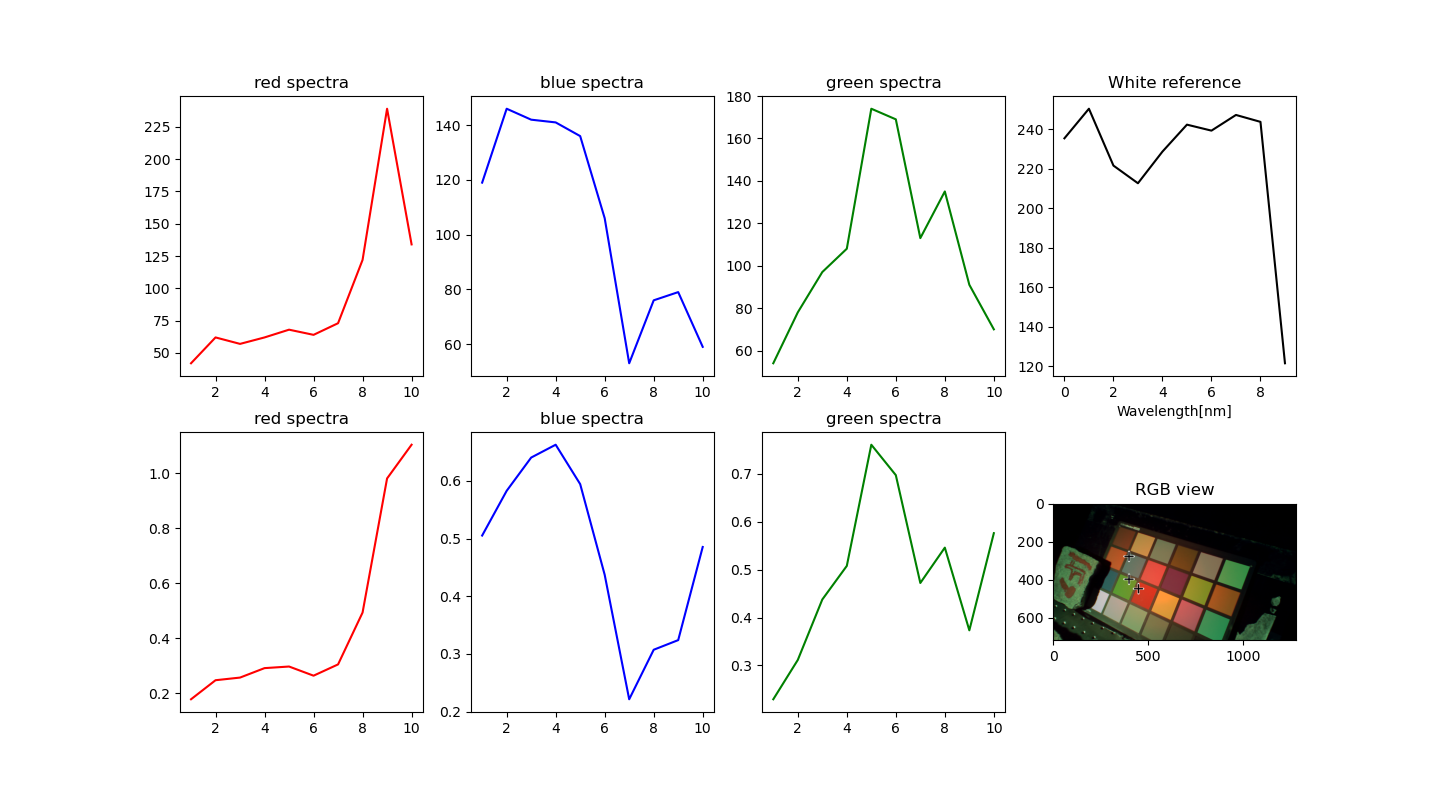
\includegraphics[width=0.75\textwidth]{./fig-task1/wc-tunable-spectra.png}
\end{figure}

Nuance image was loaded with the script shown in Code \ref{code:load-tunable}.
Figures were generated with the script shown in Code \ref{code:wc-tunable}.



\section{Tasks \#2. Nuance camera}
A spectral image by Japanese camera was loaded by the Python script
shown in Code \ref{code:load-jp}. The gray scale preview and RGB
preview are shown in Figure \ref{fig:japanese-preview}.

\begin{figure}[H]
  \centering
  \caption{Gray scale preview of Japanese camera}
  \label{fig:japanese-preview}
  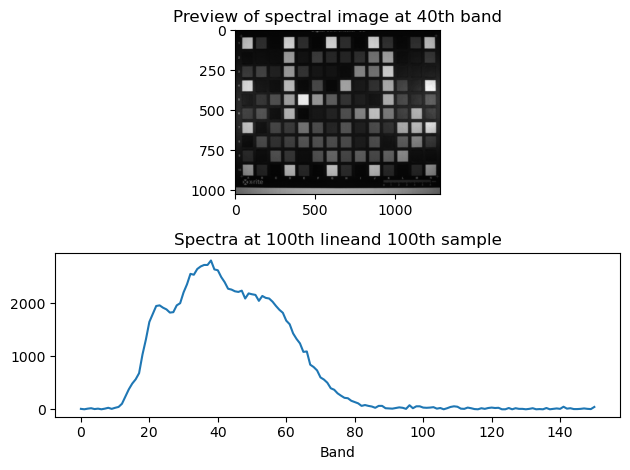
\includegraphics[width=0.5\textwidth]{./fig-task2/jp.png}
\end{figure}


\section{Tasks \#3. Build ENVI spectral image from Tunable light
source}
Tunable light sources image loaded by the function
\texttt{load\_tunable\_image} in Code \ref{code:load--tunable} is
saved in the ENVI format.
The script for saving the image is shown in Code \ref{code:save-tunable}.
The spectral image is saved as a raw file with the BIL interleave.

Preview by FreeLook software is shown in Figure \ref{fig:tunable-preview}.
\begin{figure}[H]
  \centering
  \caption{Preview of the Tunable light source image in FreeLook software}
  \label{fig:tunable-preview}
  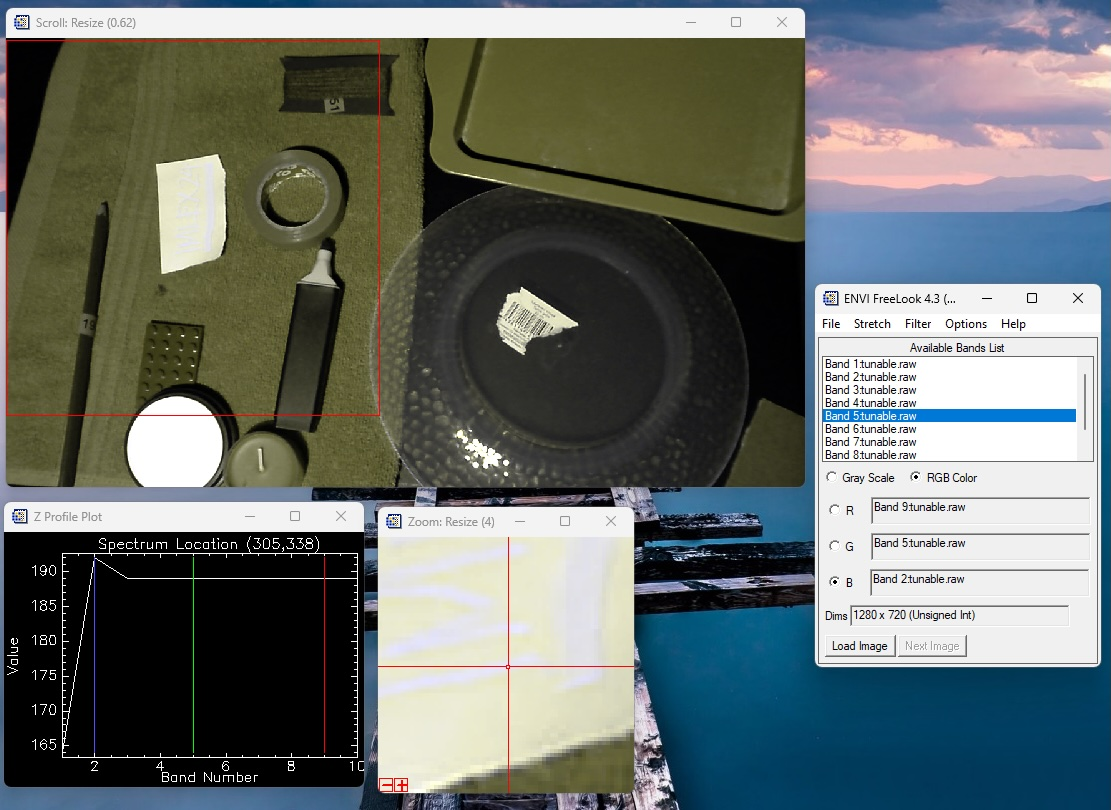
\includegraphics[width=0.5\textwidth]{./fig-task3/tunable.jpg}
\end{figure}

The header file is shown in Code \ref{code:tunable-hdr}.

\begin{lstlisting}[caption=Saved ENVI header file, label={code:tunable-hdr}]
ENVI
ENVI description = {File Imported into ENVI}
file type = ENVI
lines = 720
samples = 1280
bands = 10
interleave = bil
data type = 12
header offset = 0
byte order = 0

\end{lstlisting}


\section{Code}

The following Python scripts were used to complete the tasks. All of
those codes are available in the GitHub repository
\footnote{\url{https://github.com/8gaU8/ASI-Homeworks}}.

\begin{lstlisting}[language=python, caption=White correction for Specium Scanner, label={code:wc-specim-scanner}]
import matplotlib.pyplot as plt

from asi import path_config
from asi.draw import draw_multi_crosss, reconstruct_rgb_envi
from asi.io.load_envi import load_spectral_image
from asi.preprocess import load_white_corrected
from asi.utils import get_wavelengths

session1_root = path_config.measurements / "Session1"
spec_path = session1_root / "Specim scanner/Color_checker_8_binning/capture"

fig, axes = plt.subplots(1, 2, figsize=(10, 5))

colorchecker_path = spec_path / "solutions_scan_0110"
whiteref_path = spec_path / "WHITEREF_solutions_scan_0110"
darkref_path = spec_path / "DARKREF_solutions_scan_0110"

spectral_image, envi_header = load_spectral_image(colorchecker_path)
rgb_view = reconstruct_rgb_envi(spectral_image, envi_header)
axes[0].imshow(rgb_view)
axes[0].set_title("Before white correction")

spectral_image, envi_header = load_white_corrected(
    colorchecker_path,
    whiteref_path,
    darkref_path,
)
rgb_view = reconstruct_rgb_envi(spectral_image, envi_header)

axes[1].imshow(rgb_view)
axes[1].set_title("After white correction")
plt.show()

# Show spectra
colors = ["r", "g"]
positions = [(300, 500), (400, 1000)]
canvas = draw_multi_crosss(rgb_view, positions)

plt.rcParams["figure.dpi"] = 100
fig, axes = plt.subplots(1, 3, figsize=(10, 5), tight_layout=True)

wavelength = get_wavelengths(envi_header)
for pos, color, ax in zip(positions, colors, axes[:2]):
    ax.plot(wavelength, spectral_image[pos[1], pos[0], :], color=color)
    ax.set_title(f"Spectrum at {pos[0]}th pixel")
    ax.set_xlabel("Wavelength[nm]")

axes[2].imshow(canvas)
axes[2].set_title("RGB view of spectral image")

plt.show()
\end{lstlisting}
\begin{lstlisting}[language=python, caption=White correction for Nuance Cmaera with small reference, label={code:wc-nuance-small}]
import numpy as np
from matplotlib import pyplot as plt

from asi import path_config
from asi.draw import draw_multi_crosss, reconstruct_rgb, select_area
from asi.io.load_nuance import load_nuance_image

session1 = path_config.measurements / "session1"
nuance = session1 / "Nuance"


# White correction with small reference

fig, axes = plt.subplots(1, 2, figsize=(10, 5))
root = nuance / "colorchecker 2lights"

white_pos_list = [
    (slice(200, 300), slice(0, 50)),
    (slice(200, 300), slice(-50, -1)),
]


spectral_image, wavelengths = load_nuance_image(root)
spectral_image = spectral_image.astype(np.float64)
spectral_image /= spectral_image.max()

original_rgb = reconstruct_rgb(spectral_image, wavelengths)
for white_pos in white_pos_list:
    original_rgb = select_area(original_rgb, white_pos)
original_rgb /= original_rgb.max()
original_rgb = original_rgb.clip(0, 1)
axes[0].imshow(original_rgb)
axes[0].set_title("Before white correction")

white_sq_list = []

# White correction with selected area
for white_pos in white_pos_list:
    white_sq = spectral_image[white_pos]
    a, b, band = white_sq.shape
    white_sq = white_sq.reshape(a * b, band)

    # replace nonzero elements with minimum value
    nonzero_elements = white_sq[white_sq != 0]
    min_elm = nonzero_elements.min()
    white_sq_list.append(white_sq)

white_sq = np.vstack(white_sq_list)
whiteref = white_sq.mean(axis=0)

# spectral_image *= 1.5
# spectral_image = spectral_image.clip(0, 1)
white_corrected = spectral_image / whiteref
white_corrected /= white_corrected.max()
white_corrected = white_corrected.clip(0, 1)
del original_rgb

white_corrected_rgb_view = reconstruct_rgb(white_corrected, wavelengths)
axes[1].imshow(white_corrected_rgb_view)
axes[1].set_title("After white correction")

plt.show()

# Show spectra
colors = ["g", "r", "b"]
color_names = ["green", "red", "blue"]
positions = [(300, 500), (500, 500), (1100, 600)]


plt.rcParams["figure.dpi"] = 100
fig, axes = plt.subplots(2, 4, figsize=(10, 5), tight_layout=True)
print(axes)

axes1, axes2 = axes
for pos, color, color_name, ax in zip(positions, colors, color_names, axes2):
    print(ax)
    ax.plot(wavelengths, white_corrected[pos[1], pos[0], :], color=color)
    ax.set_title(f"Spectla at {color_name}(corrected)")
    ax.set_xlabel("Wavelength[nm]")

for pos, color, color_name, ax in zip(positions, colors, color_names, axes1):
    print(ax)
    ax.plot(wavelengths, spectral_image[pos[1], pos[0], :], color=color)
    ax.set_title(f"Spectla at {color_name}(original)")
    ax.set_xlabel("Wavelength[nm]")


axes1[-1].plot(wavelengths, whiteref, color="k")
axes1[-1].set_title("White reference")
axes1[-1].set_xlabel("Wavelength[nm]")

canvas = draw_multi_crosss(white_corrected_rgb_view, positions)
axes2[-1].imshow(canvas)
axes2[-1].set_title("RGB view")

plt.show()
\end{lstlisting}
\begin{lstlisting}[language=python, caption=White correction for Nuance Cmaera with large reference, label={code:wc-nuance-large}]
import numpy as np
from matplotlib import pyplot as plt

from asi import path_config
from asi.draw import draw_multi_crosss, reconstruct_rgb, select_area
from asi.io.load_nuance import load_nuance_image

session1 = path_config.measurements / "session1"
nuance = session1 / "Nuance"

# White correction with large reference

# load white image

root = nuance / "white 2lights"

white_image, wavelengths = load_nuance_image(root)
white_image = white_image.astype(np.float64)


fig, axes = plt.subplots(1, 2, figsize=(10, 5))

white_pos = (slice(200, 1000), slice(200, 1200))


white_rgb = reconstruct_rgb(white_image, wavelengths)
white_rgb = select_area(white_rgb, white_pos)
white_rgb /= white_rgb.max()
white_rgb = white_rgb.clip(0, 1)
axes[0].imshow(white_rgb)
axes[0].set_title("Before white correction")


# White correction with selected area
white_sq = white_image[white_pos]

# replace nonzero elements with minimum value
nonzero_elements = white_sq[white_sq != 0]
min_elm = nonzero_elements.min()
white_sq = white_sq.clip(min_elm, None)


# load spectral image
root = nuance / "colorchecker 2lights"
spectral_image, wavelengths = load_nuance_image(root)

# apply white correction
whiteref = white_sq.mean((0, 1))
white_corrected = spectral_image / whiteref
white_corrected /= white_corrected.max()
white_corrected = white_corrected.clip(0, 1)
del white_rgb

white_corrected_rgb_view = reconstruct_rgb(white_corrected, wavelengths)
axes[1].imshow(white_corrected_rgb_view)
axes[1].set_title("After white correction")

plt.show()

# Show spectra
colors = ["g", "r", "b"]
color_names = ["green", "red", "blue"]
positions = [(300, 500), (500, 500), (1100, 600)]


plt.rcParams["figure.dpi"] = 100
fig, axes = plt.subplots(2, 4, figsize=(10, 5), tight_layout=True)
print(axes)

axes1, axes2 = axes
for pos, color, color_name, ax in zip(positions, colors, color_names, axes2):
    print(ax)
    ax.plot(wavelengths, white_corrected[pos[1], pos[0], :], color=color)
    ax.set_title(f"Spectla at {color_name}(corrected)")
    ax.set_xlabel("Wavelength[nm]")

for pos, color, color_name, ax in zip(positions, colors, color_names, axes1):
    print(ax)
    ax.plot(wavelengths, spectral_image[pos[1], pos[0], :], color=color)
    ax.set_title(f"Spectla at {color_name}(original)")
    ax.set_xlabel("Wavelength[nm]")


axes1[-1].plot(wavelengths, whiteref, color="k")
axes1[-1].set_title("White reference")
axes1[-1].set_xlabel("Wavelength[nm]")

canvas = draw_multi_crosss(white_corrected_rgb_view, positions)
axes2[-1].imshow(canvas)
axes2[-1].set_title("RGB view")

plt.show()

\end{lstlisting}

\begin{lstlisting}[language=python, caption=Load Nuance Cmaera, label={code:load-nuance}]
from pathlib import Path

import numpy as np
import tifffile as tiff
from natsort import natsorted

def load_nuance_image(tiff_root: Path) -> tuple[np.ndarray, list[float]]:
    wavelengths: list[float] = []
    imgs = []
    tiff_list = list(tiff_root.glob("*.tif"))
    tiff_list = natsorted(tiff_list, reverse=False)
    for tiff_path in tiff_list:
        img = tiff.imread(tiff_path)
        wavelength = float(tiff_path.stem.split("_")[-1])
        imgs.append(img)
        wavelengths.append(wavelength)

    spectral_image = np.stack(imgs, axis=-1)
    spectral_image = spectral_image.astype(np.float64)
    return spectral_image, wavelengths

\end{lstlisting}

\begin{lstlisting}[language=python, caption=Load ENVI format images, label={code:load-envi}]
from pathlib import Path

import numpy as np

def parse_envi_header(lines: list) -> dict[str, str]:
    """
    Parses ENVI file content into a structured dictionary
    This code was written with Github Copilot
    """
    envi_data = {}
    in_block_key = None

    for line_org in lines:
        line = line_org.strip()

        # Skip empty lines
        if not line:
            continue

        # Handle multiline blocks
        if in_block_key:
            if line.endswith("}"):
                # Closing multiline
                envi_data[in_block_key] += line[:-1].strip()
                in_block_key = None
            else:
                # Continue multiline
                envi_data[in_block_key] += line
            continue

        # Key-value pair parsing
        if "=" in line:
            key, value = map(str.strip, line.split("=", 1))
            key = key.lower().replace(" ", "_")  # Normalize key format

            # Handle block values
            if value.startswith("{"):
                # Handle multiline block
                in_block_key = key
                # Remove opening '{'
                value = value[1:].strip()
                if value.endswith("}"):
                    # Single-line block
                    envi_data[key] = value[:-1]
                    in_block_key = None
                else:
                    # Start multiline block
                    envi_data[key] = value
            else:
                # Single-line value
                envi_data[key] = value
    return envi_data

def load_envi_header(hdr_file: Path) -> dict[str, str]:
    """Loads ENVI header file."""
    with hdr_file.open(encoding="utf-8") as f:
        header_content = f.readlines()
    envi_header = parse_envi_header(header_content)
    return envi_header

def load_spectral_image(file_stem: Path) -> tuple[np.ndarray, dict[str, str]]:
    """Loads spectral image from ENVI format."""
    # Load ENVI header
    hdr_file = file_stem.with_suffix(".hdr")
    envi_header = load_envi_header(hdr_file)

    # Load parameters
    interleave = str(envi_header["interleave"])
    lines = int(envi_header["lines"])
    samples = int(envi_header["samples"])
    bands = int(envi_header["bands"])
    data_type = int(envi_header.get("data type", 12))

    # Map ENVI data type to NumPy dtype
    data_type_map = {
        1: np.uint8,
        2: np.int16,
        3: np.int32,
        4: np.float32,
        5: np.float64,
        6: np.complex64,
        9: np.complex128,
        12: np.uint16,
        13: np.uint32,
        14: np.int64,
        15: np.uint64,
    }

    if data_type not in data_type_map:
        msg = f"Unsupported data type: {data_type}"
        raise ValueError(msg)

    dtype = data_type_map[data_type]

    # Load raw data
    raw_file = file_stem.with_suffix(".raw")
    with open(raw_file, "rb") as f:
        raw = np.fromfile(f, dtype=dtype)

    # define shape and transpose order by interleave method
    if interleave.upper() == "BIL":
        new_shape = (lines, bands, samples)
        axis_order = (0, 2, 1)
    elif interleave.upper() == "BIP":
        new_shape = (lines, samples, bands)
        axis_order = (0, 1, 2)
    elif interleave.upper() == "BSQ":
        new_shape = (bands, samples, lines)
        axis_order = (0, 2, 1)
    else:
        msg = f"Interleave {interleave} not supported."
        raise ValueError(msg)

    spectral_image = raw.reshape(new_shape)
    # change axis order to 'lines, samples, bands'
    spectral_image = np.transpose(spectral_image, axis_order)

    return spectral_image, envi_header

\end{lstlisting}
\begin{lstlisting}[language=python, caption=White correction for SpecimIQ with small reference, label={code:wc-specimiq-small}]
import numpy as np
from matplotlib import pyplot as plt

from asi import path_config
from asi.draw import draw_multi_crosss, reconstruct_rgb_envi, select_area
from asi.io.load_envi import load_spectral_image
from asi.preprocess import load_white_corrected
from asi.utils import get_wavelengths

specim_iq_root = path_config.measurements / "Session1" / "SpecimIQ"

path_404 = specim_iq_root / "404" / "capture"

# White correction with small reference
fig, axes = plt.subplots(1, 2, figsize=(10, 5))

image_path = path_404 / "404"
spectral_image, envi_header = load_spectral_image(image_path)

white_pos_list = [
    (slice(65, 102), slice(332, 370)),
    (slice(400, 430), slice(370, 400)),
]

original_rgb = reconstruct_rgb_envi(spectral_image, envi_header)
for white_pos in white_pos_list:
    original_rgb = select_area(original_rgb, white_pos)

original_rgb *= 1.5
original_rgb = original_rgb.clip(0, 1)

axes[0].imshow(original_rgb)
axes[0].set_title("Before white correction")

# White correction with selected area
white_sq_list = []
for white_pos in white_pos_list:
    white_sq = spectral_image[white_pos]
    a, b, band = white_sq.shape
    white_sq = white_sq.reshape(a * b, band)

    # replace nonzero elements with minimum value
    nonzero_elements = white_sq[white_sq != 0]
    min_elm = nonzero_elements.min()
    white_sq_list.append(white_sq)

white_sq = np.vstack(white_sq_list)
whiteref = white_sq.mean(axis=0)

white_corrected = spectral_image / whiteref

white_corrected_rgb_view = reconstruct_rgb_envi(white_corrected, envi_header)
white_corrected_rgb_view *= 1.5
white_corrected_rgb_view = white_corrected_rgb_view.clip(0, 1)

axes[1].imshow(white_corrected_rgb_view)
axes[1].set_title("After white correction")

plt.show()

# Show spectra
colors = ["r", "b", "g"]
color_names = ["red", "blue", "green"]
positions = [(320, 320), (320, 420), (320, 380)]

wavelengths = get_wavelengths(envi_header)

fig, axes = plt.subplots(2, 4, figsize=(10, 5), tight_layout=True)

axes1, axes2 = axes
for pos, color, color_name, ax in zip(positions, colors, color_names, axes2):
    ax.plot(wavelengths, white_corrected[pos[1], pos[0], :], color=color)
    ax.set_title(f"Spectra at {color_name}(corrected)")
    ax.set_xlabel("Wavelength[nm]")

for pos, color, color_name, ax in zip(positions, colors, color_names, axes1):
    ax.plot(wavelengths, spectral_image[pos[1], pos[0], :], color=color)
    ax.set_title(f"Spectra at {color_name}(original)")
    ax.set_xlabel("Wavelength[nm]")

axes1[-1].plot(wavelengths, whiteref, color="k")
axes1[-1].set_title("White reference")
axes1[-1].set_xlabel("Wavelength[nm]")

canvas = draw_multi_crosss(white_corrected_rgb_view, positions)
axes2[-1].imshow(canvas)
axes2[-1].set_title("RGB view")

plt.show()

\end{lstlisting}

\begin{lstlisting}[language=python, caption=White correction for SpecimIQ with large reference, label={code:wc-specimiq-large}]
from matplotlib import pyplot as plt

from asi import path_config
from asi.draw import draw_multi_crosss, reconstruct_rgb_envi, select_area
from asi.io.load_envi import load_spectral_image
from asi.utils import get_wavelengths

specim_iq_root = path_config.measurements / "Session1" / "SpecimIQ"

# White correction with small reference
fig, axes = plt.subplots(1, 3, figsize=(15, 5))

image_path = specim_iq_root / "404" / "capture" / "404"
spectral_image, envi_header = load_spectral_image(image_path)

original_rgb = reconstruct_rgb_envi(spectral_image, envi_header)

# original_rgb *= 1.5
# original_rgb = original_rgb.clip(0, 1)

axes[0].imshow(original_rgb)
axes[0].set_title("Before white correction")

white_path = specim_iq_root / "405" / "capture" / "405"
white_image, white_envi_header = load_spectral_image(white_path)

white_pos = (slice(200, 480), slice(100, 380))
white_rgb_view = reconstruct_rgb_envi(white_image, white_envi_header)
white_rgb_view = select_area(white_rgb_view, white_pos)

axes[1].imshow(white_rgb_view)
axes[1].set_title("Selected white area")

white_sq = white_image[white_pos]

# White correction with selected area
whiteref = white_sq.mean(axis=(0,1))

white_corrected = spectral_image / whiteref

white_corrected_rgb_view = reconstruct_rgb_envi(white_corrected, envi_header)
# white_corrected_rgb_view *= 2.5
# white_corrected_rgb_view = white_corrected_rgb_view.clip(0, 1)

axes[2].imshow(white_corrected_rgb_view)
axes[2].set_title("After white correction")

plt.show()

# Show spectra
colors = ["r", "b", "g"]
color_names = ["red", "blue", "green"]
positions = [(320, 320), (320, 420), (320, 380)]

wavelengths = get_wavelengths(envi_header)

fig, axes = plt.subplots(2, 4, figsize=(10, 5), tight_layout=True)

axes1, axes2 = axes
for pos, color, color_name, ax in zip(positions, colors, color_names, axes2):
    ax.plot(wavelengths, white_corrected[pos[1], pos[0], :], color=color)
    ax.set_title(f"Spectra at {color_name}(corrected)")
    ax.set_xlabel("Wavelength[nm]")

for pos, color, color_name, ax in zip(positions, colors, color_names, axes1):
    ax.plot(wavelengths, spectral_image[pos[1], pos[0], :], color=color)
    ax.set_title(f"Spectra at {color_name}(original)")
    ax.set_xlabel("Wavelength[nm]")

axes1[-1].plot(wavelengths, whiteref, color="k")
axes1[-1].set_title("White reference")
axes1[-1].set_xlabel("Wavelength[nm]")

canvas = draw_multi_crosss(white_corrected_rgb_view, positions)
axes2[-1].imshow(canvas)
axes2[-1].set_title("RGB view")

plt.show()

\end{lstlisting}
\begin{lstlisting}[language=python, caption=Load Tunable Light Sources images, label={code:load-tunable}]
from pathlib import Path

import cv2
import numpy as np

# CONSTS
MAX_PIXEL_VALUE = 255
MIN_PIXEL_VALUE = 0

def parse_png_path(path: Path) -> tuple[str, int, float]:
    # parse path of tunable files
    path_parts = path.stem.split(",")
    name = path_parts[0]
    ch_info = path_parts[1]
    exp_info = path_parts[2]
    ch_id = int(ch_info.strip().split(" ")[1])
    exp_id = float(exp_info.strip().split(" ")[1])
    return name, ch_id, exp_id

def gen_template(name: str, ch: int) -> str:
    return f"{name}, ch {ch}, exp * ms.png"

def get_score(im: np.ndarray) -> int:
    nb_max = (im == MAX_PIXEL_VALUE).sum()
    nb_min = (im == MIN_PIXEL_VALUE).sum()
    return nb_max + nb_min

def load_tunable_image(
    tunable_root: Path, name: str, white_pos: tuple[slice, slice]
) -> tuple[np.ndarray, list[int]]:
    png_list = list(tunable_root.glob("*.png"))
    channels = {parse_png_path(p)[1] for p in png_list}
    channels = sorted(channels)
    imgs = []
    # chose minimum score image
    for ch in channels:
        best_im = None
        best_score = 1e9
        template = gen_template(name, ch)
        for png_path in tunable_root.glob(template):
            # Select minimum score image. Score is calculated from number of unvalid pixels
            im = cv2.imread(str(png_path), cv2.IMREAD_GRAYSCALE)
            if im[white_pos].max() == MAX_PIXEL_VALUE:
                continue
            score = get_score(im)
            if score < best_score:
                best_score = score
                best_im = im
        if best_im is None:
            msg = f"Channel {ch} not found."
            raise ValueError(msg)
        imgs.append(best_im)

    spectral_image = np.stack(imgs, axis=-1)
    return spectral_image, channels

\end{lstlisting}

\begin{lstlisting}[language=python, caption=White correction for Tunable Light Sources with small white reference, label={code:wc-tunable}]
import matplotlib.pyplot as plt
import numpy as np

from asi import path_config
from asi.draw import draw_multi_crosss, select_area
from asi.io import load_tunable_image

# Configurations
WHITE_POS = (slice(510, 550), slice(230, 260))
SELECT_CHANNELS = [9, 4, 0]
# LOAD IMAGE
session1 = path_config.measurements / "session1"
tunable_root = session1 / "Tunable light sorces" / "ImagesASI"

spectral_image, channels = load_tunable_image(
    tunable_root, name="colorchecker", white_pos=WHITE_POS
)
spectral_image = spectral_image.astype(np.float64)

# Make RGB view
rgb_view = spectral_image[..., SELECT_CHANNELS]
# Postprocess for preview
rgb_view /= rgb_view.max()
rgb_view *= 0.8
rgb_view = rgb_view.clip(0, 1)

# Select white area for correction
rgb_view = select_area(rgb_view, WHITE_POS)

# Apply white correction
white_sq = spectral_image[WHITE_POS]
whiteref = white_sq.mean(axis=(0, 1))
white_corrected = spectral_image / whiteref

# RGB view after white correction
white_corrected_rgb_view = white_corrected[..., SELECT_CHANNELS]
white_corrected_rgb_view /= white_corrected_rgb_view.max()
white_corrected_rgb_view *= 1.2
white_corrected_rgb_view = white_corrected_rgb_view.clip(0, 1)

# Plot images
fig, axes = plt.subplots(1, 2, figsize=(10, 5))
axes[0].imshow(rgb_view)
axes[0].set_title("Before white correction")

axes[1].imshow(white_corrected_rgb_view)
axes[1].set_title("After white correction")

plt.show()

# show spectra
red_pos = (450, 450)
blue_pos = (400, 280)
green_pos = (400, 400)

pos_list = (red_pos, blue_pos, green_pos)
colors = ["r", "b", "g"]
color_names = ["red", "blue", "green"]

fig, axes = plt.subplots(2, 4, figsize=(15, 8))

org_axes, white_axes = axes
for axes, image in zip([org_axes, white_axes], [spectral_image, white_corrected]):
    for pos, color_name, color, ax in zip(pos_list, color_names, colors, axes):
        ax.plot(channels, image[pos[1], pos[0], :], color=color)
        ax.set_title(f"{color_name} spectra")

org_axes[-1].plot(whiteref, color="k")
org_axes[-1].set_title("White reference")
org_axes[-1].set_xlabel("Wavelength[nm]")

canvas = draw_multi_crosss(white_corrected_rgb_view, pos_list)
white_axes[-1].imshow(canvas)
white_axes[-1].set_title("RGB view")

plt.show()
\end{lstlisting}
\begin{lstlisting}[language=python, caption=Save nuance image as ENVI format, label={code:save-nuance}]
from pathlib import Path

import numpy as np

from asi import path_config
from asi.io.load_nuance import load_nuance_image

session1 = path_config.measurements / "session1"
nuance = session1 / "Nuance"

root = nuance / "colorchecker 2lights"
spectral_image, wavelengths = load_nuance_image(root)

lines, samples, bands = spectral_image.shape
print(spectral_image.shape)
spectral_image_uint16 = (spectral_image).astype(np.uint16)
bil_format = spectral_image_uint16.transpose(0, 2, 1).flatten()

bil_format.tofile("saveddata/nuance.raw")

reversed_wavelengths = wavelengths[::-1]
wavelengths_hdr = ",\n\t".join(map(str, reversed_wavelengths))
wavelengths_hdr = f"wavelength = {{\n\t{wavelengths_hdr}\n}}"

header_content = f"""ENVI
ENVI description = {{File Imported into ENVI}}
file type = ENVI
lines = {lines}
samples = {samples}
bands = {bands}
interleave = bil
data type = 12
header offset = 0
byte order = 0
{wavelengths_hdr}
"""

hdr_dst_path = Path("saveddata/nuance.hdr")
hdr_dst_path.write_text(header_content, encoding="utf-8")
\end{lstlisting}
